% !TeX root = ./thesis.tex










%==============================
\chapter{Introduction}
\label{chap:introduction}


%-----
%\section{Motivation}
\markright{Motivation}
\EBlettrine{One} might ask what flocks of birds, schools of fish, herds of ungulates, swarms of insects, mexican waves, mosh pits, the stock exchange and biological cells have in common? They are all examples of collective (animal) behaviour (see \figurename~\ref{fig:CB}). The study of collective behaviour is fascinating as it analyses how simple actions of an individual influence the complex dynamics of a group. Aristotle once stated, ``The whole is more than the sum of its parts.'' -- a statement that describes the essence of collective behaviour. Because the phenomenon is so widespread results from studies of collective behaviour are useful for scientists from many different research fields -- from biology, physics, and medicine, to social studies, computer science, and control theory \cite{deisboeck2009collective,lebarbajec2009organized,nahin2012chases,silverberg2013collective,spector2003emergence,sumpter2006principles,vicsek1995novel,wei2009pursuit,xu2014crowd}.

\begin{figure}[p]
	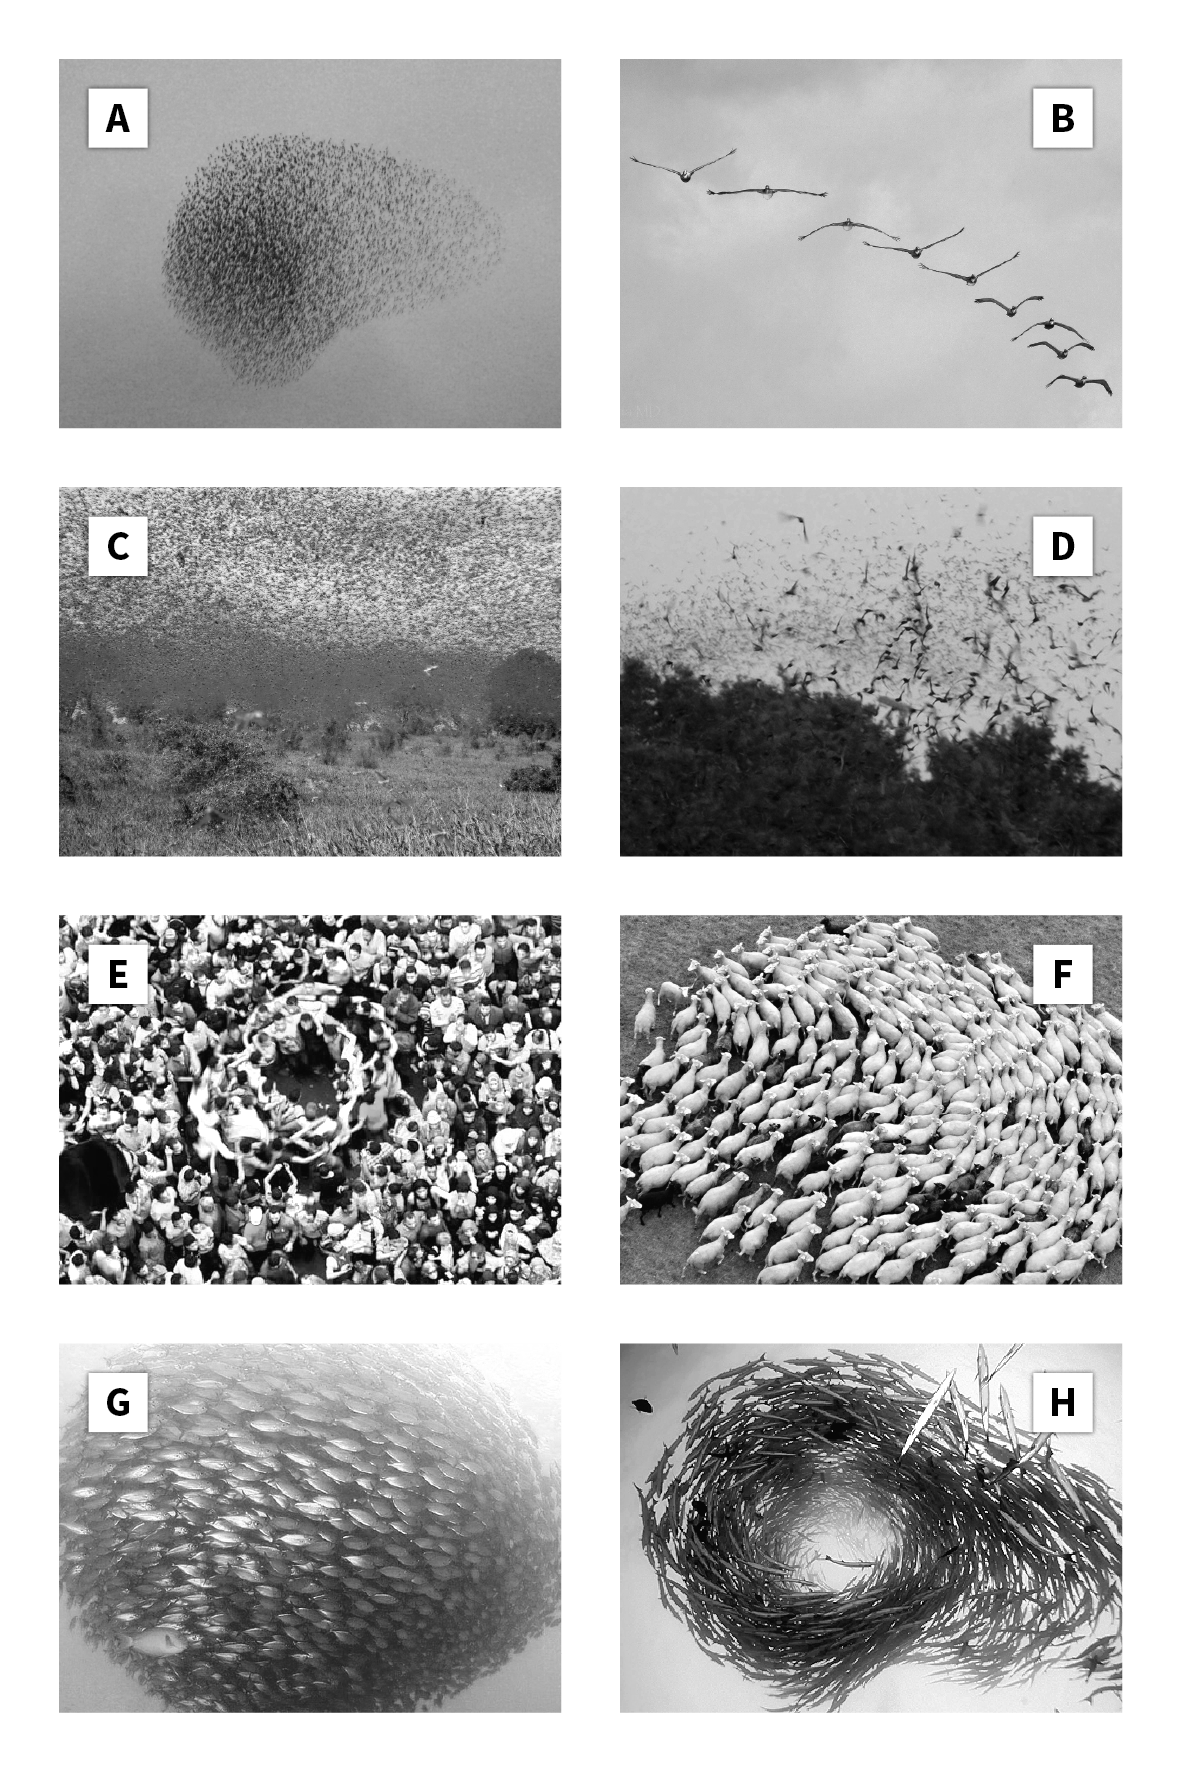
\includegraphics[width=\figurewidth]{figCB_BW}
	\caption{Examples of various forms of collective behaviour found in nature. A) a murmuration of stralings (© Tim Regan, \href{http://www.flickr.com}{flickr.com}). B) a squadron of pelicans flying in formation (© Daniel D'Auria, \href{http://www.flickr.com}{flickr.com}). C) a swarm of locusts (© FAO emergencies, \href{http://www.flickr.com}{flickr.com}). D) a swarm of bats (© Amanda, \href{http://www.flickr.com}{flickr.com}). E) a mosh pit on a rock concert (© Amanda Mustard, \href{http://www.amandamustard.com/}{amandamustard.com}). F) a herd of sheep (© Dariusz Paciorek, \href{http://www.aeroart.com.pl/}{aeroart.com.pl}). G) the bait ball phenomenon (© Bo Pardau, \href{http://www.flickr.com}{flickr.com}). H) milling fish (© Robin Hughes, \href{http://www.flickr.com}{flickr.com}).}
	\label{fig:CB}
\end{figure}

The collective behaviour research field (in certain research communities known also by the names collective animal behaviour or swarm behaviour) is very active as even though the phenomenon can be easily observed in nature, many scientific questions remain unanswered \cite{krause2002living,lebarbajec2009organized,sumpter2006principles}. In the biological community examples of such questions are why groups, especially organized ones, form in the first place, and why we see so much variation in behaviour \cite{lebarbajec2009organized}. For example, why do so few bird species that fly together display organized behaviour, and why do even closely related species \cite{jarvis2014wholegenome} display major differences in flocking behaviour \cite{lebarbajec2009organized}? The literature about collective behaviour contains several different and sometimes contradictory hypotheses about why animals coalesce into groups. Some studies advocate that aggregations boost mating and foraging efficiency \cite{krebs1994behavioural}, others claim that fish and birds in highly organized groups save energy because of hydrodynamic or aerodynamic benefits \cite{hemelrijk2014increased,marras2015fish,portugal2014upwash}.

Probably the most common hypotheses about the origins of collective behaviour state that grouping functions as an effective defence against predators \cite{cresswell2011predicting,hart2005predator,krause2002living,larsson2012why,lebarbajec2009organized,nishimura2002predator,pavlov2000patterns}. The \emph{selfish herd} hypothesis \cite{hamilton1971geometry} suggests that animals form groups in order to reduce their domain of danger -- an area surrounding an individual in which all points within that area are closer to the observed individual than to any other \cite{viscido2001response}. The \emph{dilution of risk} hypothesis suggests that the chance of a single prey being selected as the predator's target is lower in larger groups \cite{tosh2011conditions}. The \emph{many eyes} hypothesis suggests that as the size of the group increases the probability of detecting a predator also increases \cite{galton1871gregariousness} and the amount of time individuals in the group need to be vigilant against predators decreases \cite{elgar1989predator,haley2014exploring,ruxton2008application,sadedin1998influence}, giving them more time for other tasks (\eg foraging). Last but not least, the \emph{confusion hypothesis} states that a predator attacking a group of visually similar prey might have a hard time tracking and capturing its target \cite{demsar2015simulating,kunz2006prey,nishimura2002predator,olson2013predator,olson2016evolution,zheng2005behavior}.

Some manifestations of collective behaviour (\eg schools of fish and flocks of birds) are quite large in scale and as such hard to enclose in a controlled environment in which scientists could then test the hypotheses about the ``whys'' and ``hows'' of such behaviour \cite{lebarbajec2009organized}. In addition in nature different predators with different hunting tactics exist in different environments, meaning that it is difficult to compare the effects of predation pressures on the behaviour without the confounding effects of environmental context. With computational approaches one can develop models that reproduce the studied behaviour and at the same time diminish the confounding effects of the environment. It comes as no surprise then that computational approaches are a more and more frequently used tool for studying various hypotheses concerning collective behaviour \cite{vicsek1995novel,couzin2002collective,hildenbrandt2010selforganized}. Because computational approaches give scientists full control over the involved parameters, the results are usually also not species specific but more general.

%-----
\section{Individual-based models}

There are two prominent computational approaches suitable for studying collective behaviour. The first one is called Eulerian modelling, which typically uses partial differential equations to describe the flux of a property -- how that property changes through time and space. In the case of collective behaviour studies the property in question is usually population density \cite{kunz2011implications}. However, Eulerian modelling has two weaknesses, the individual variations (\eg in speed, body size, vision, etc.) cannot be easily incorporated \cite{gautrais2008keybehavioural}, and it does not allow to trace the properties on the group level back to the behaviour of individuals \cite{deangelis2005individualbased}. Eulerian modelling can thus be interpreted as a top-down approach to modelling collective behaviour, where one single equation is sought, an equation which describes the dynamics of the property in question on a global level. Needless to say, Eulerian modelling is suitable for tackling with research questions related to the global properties of collective behaviour assuming that one exists; questions related to how or why such behaviour emerges, on the other hand, are extremely difficult or impossible to answer.

Because of these reasons the most common computational approach to the study of collective behaviour is the so called individual-based modelling (also known as Lagrangian modelling, or agent-based modelling). The reasoning behind such modelling is that to be able to address questions related to how or why collective behaviour emerges the focus should be on the individual, and thus the approach can be viewed also as a bottom-up approach to modelling collective behaviour. In individual-based models the behaviour of each individual is defined by its local algorithm (local program). A local algorithm describes how an individual reacts to its neighbours, nearby environment, and possibly its own internal state. Once researches define the behaviour (reactions) of individuals they run computer simulations where many of these individuals reside in a shared environment. In these simulations, the behaviour of individuals results from local interactions and is usually calculated in turn for each individual and integrated over time. During simulations researchers observe and try to explain the patterns that emerge on a group level via local interactions \cite{grimm1999tenyears}. In other words, researchers program the behaviour of individuals (local level) and then observe the behaviour at the global level that emerges from interactions at the local level \cite{dewolf2005emergence}. In individual-based models there is usually no central or external mechanism that would impose order and structure on the global level. The emergence of order and structure from local interactions on the global level is also known as \emph{self-organization}. Self-organization is a very interesting research topic on its own as besides biological systems (\eg animal aggregations) it exists also in the world of physics (\eg Rayleigh-B{\'e}nard convection cells \cite{getling1998rayleigh}) and chemistry (\eg Belousov–Zhabotinsky reaction \cite{zhabotinsky1964periodic}). An interesting, but rather unconventional approach used for the study of self-organizing patterns is \emph{amorphous computing} \cite{abelson1996amorphous,abelson2000amorphous}, which builds computational systems made from very large numbers of identical, parallel processors each having limited computational ability and local interactions. For example, Coore \cite{coore1994botanical} demonstrated that local entities in amorphous computing can be configured to generate pre-specified patterns that resemble self-organization.

In biological studies devoted to answering questions why or how collective behaviour emerges, most often the individual-based models for simulating the motion of groups of animals are designed by hand. In such hand-crafted, or pre-set, models the behaviour of artificial animals, or \emph{animats} \cite{cliff1993adding,fine2013unifying,lebarbajec2005fuzzy,watts1998animats,wilson1985knowledge}, is designed by the researchers/programmers and then fine-tuned to as closely as possible mimic the behaviour of animals in nature \cite{couzin2002collective,demsar2014simulated,demsar2015simulating,lebarbajec2005fuzzy,lebarbajec2005simulating,hildenbrandt2010selforganized,vicsek1995novel}. When fine-tunning and validating the researchers resort to various metrics by which they compare the behaviour of animats to the behaviour of the modelled animals. The developed models (designed and fine-tuned) are then used to study the behaviour of animals by simulating various situations in a controlled environment and observing the reactions and interactions of large numbers of animats.

%-----
\section{The animat}

The animat can be defined as a Moore automaton \cite{kohavi1978switching} with a three stage transition function (see Definition~\ref{def:animat} and \figurename~\ref{fig:animat}) \cite{lebarbajec2003boids,lebarbajec2003fuzzifying,lebarbajec2005fuzzy,lebarbajec2007boids}. It abstracts the basic characteristics of a real animal. Just like a real animal, it exists in time and space and is surrounded by inanimate and animate objects (\ie the \emph{universe}). It is aware of its current state and capable of \emph{perceiving} the state of the universe. By performing \emph{actions}, governed by its \emph{drives}, the animat is capable of influencing its own state and the state of the universe \cite{lebarbajec2005fuzzy}.

\begin{definition}
	\label{def:animat}
	An animat $\autom{A}=\langle\set{X},\set{Q},\set{Y},\delta,\lambda,P,D,S\rangle$ is an extended Moore automaton, where $\set{X}$, $\set{Q}$ and $\set{Y}$ are non-empty sets representing the input alphabet, the internal states and the output alphabet respectively; $\delta: \set{X}\times \set{Q}\rightarrow \set{Q}$ is a mapping called the transition function and $\lambda: \set{Q}\rightarrow \set{Y}$ is a mapping called the output function. At any discrete time step $t \in \set{T}$, where $\set{T}$ is a non-empty set of discrete time steps, the automaton is in a state $q_t \in \set{Q}$. The state determines the future input-output behaviour. If an input $x_t \in \set{X}$ is applied, then, in the next discrete time step $t+1$, the automaton assumes a new state $q_{t+1} = \delta(x_t,q_t)$ that depends both on the current state and the input. In addition, the automaton emits the output $\lambda(q_{t+1}) \in \set{Y}$, which depends on the new state.	
	In the case of the animat its input in a given discrete time step is the perceived state of the universe (a collection of animats) at the same time step and for that reason its input alphabet is $\set{X}=\set{Y}_1 \times \cdots \times \set{Y}_n$, where $\set{Y}_1,\ldots,\set{Y}_n$ are output alphabets of the $n$ animats that represent the universe. In addition $P=\langle P_1,\ldots,P_k\rangle$, $D=\langle D_1,\ldots,D_l\rangle$, and $S$ are a $k$-tuple of perception functions, an $l$-tuple of drive functions, and an action selection function respectively and the transition function $\delta$ is defined as:
	\begin{eqnarray}
		& p_i = P_i(x,q),\ i=1,\ldots,k, & \\
		& a_j = D_j(\langle p_1,...,p_k\rangle,q),\ j=1,\ldots,l, & \\
		& \delta(x,q) = S(\langle a_1,...,a_l\rangle,q). &
	\end{eqnarray}
\end{definition}

\begin{figure}
	\vskip.2in % add some top and bottom whitespace
	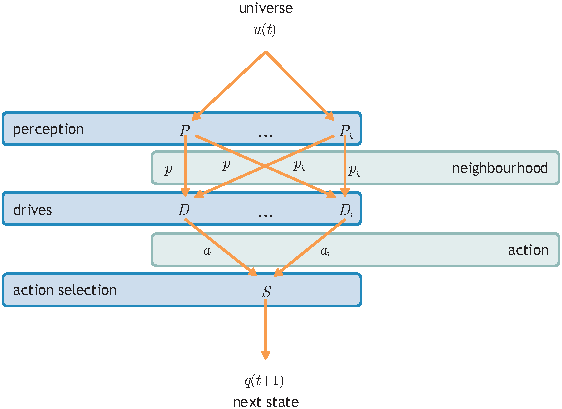
\includegraphics[width=.6\figurewidth]{fig[animat]}
	\vskip.2in
	\caption{A visual representation of the processes and terminology associated with an artificial animal, the animat.}
	\label{fig:animat}
\end{figure}

As animals in nature are able to monitor their surroundings via their senses (sight, lateral line, hearing, etc.), animats are able to perceive their \emph{neighbourhood}, the current state of the universe nearby. Animats continuously attempt to optimise the rate of occurrences of events that will fulfil their drives. Drives in animats thus imitate the instinctive needs that make real animals tick and perform actions that are necessary to survive in their natural habitat. A few examples of such drives are: the drive to feed, the drive to mate, social drives, etc. More often than not there is no ``one action to rule them all,'' meaning that there is no single action that could satisfy all of the animat's drives at the same time. For example, let us consider a hungry animal with a feeding area nearby. If there are no predators roaming around the feeding area, the decision of the animal (action selection) is trivial -- move towards the food. If there are predators nearby, however, the animal's decision becomes a bit more complicated as it has to meld the actions that will satisfy the drive to feed with those that will satisfy the drive to flee. If the animal is facing the threat of dying by starvation it might decide to move towards the food despite the danger of being eaten by a predator. On the other hand, if it is just slightly hungry it might decide that a better option would be to try and find a different source of food, a source of food that does not have predators lurking around. Therefore, the animat has to perform some kind of \emph{action selection} in order to appease its drives. In other words the action selection tries to satisfy as many of the animat's drives as posible given the animat's current state and the state of the universe nearby.

With individual-based models it has been demonstrated that complex collective behaviour can emerge if individuals follow relatively simple drives. The first attempts at modelling collective behaviour via individual-based models were made in the 1980s. Aoki \cite{aoki1982simulation} proposed a bottom-up approach to the simulation of schooling mechanisms in fish. Reynolds \cite{reynolds1987flocks} presented the first computer model for procedural animation of flocking birds. Heppner \& Grenander \cite{heppner1990stochastic}, working on a similar project, modelled the behaviour of birds with stochastic non-linear differential equations. These and subsequent individual-based models \cite{couzin2002collective,demsar2013family,demsar2014simulated,demsar2015simulating,demsar2016balanced,demsar2017evolution,helbing1995social,hildenbrandt2010selforganized,lebarbajec2009organized,parrish2002schools,schellinck2011review,sumpter2006principles,vicsek2012collective} differ in the way they implement individual parts, but in most models the behaviour is a constant blending of three drives called \emph{cohesion}, \emph{separation}, and \emph{alignment} (see \figurename~\ref{fig:drives}). Cohesion denotes the attraction toward other individuals and is usually modelled as the tendency to move towards distant individuals when there are none nearby; separation models the tendency to move away from neighbours that are too close, to avoid collisions. The third drive, alignment, models the tendency to synchronize velocity (direction and speed of movement) with nearby neighbours. As a perfect synchronization of movements will prevent collisions and lead to the formation of groups the alignment drive can be interpreted also as a passive form of avoidance and attraction, and due to this some models concentrate exclusively on the alignment drive \cite{vicsek1995novel}.

\begin{figure*}
	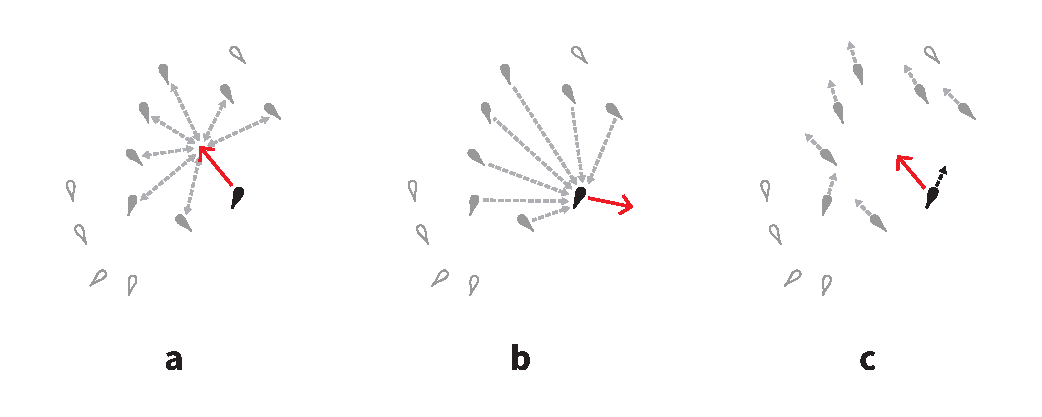
\includegraphics[width=\figurewidth]{figDrives}
	\caption{Visualization of the three basic drives: (a) cohesion, (b) separation, and (c) alignment. The black animat is the observed individual. The grey animats are the perceived neighbours that influence the observed animat's behaviour. The white and outlined animats are neighbours that have no direct influence on the observed animat's behaviour.}
	\label{fig:drives}
\end{figure*}

%-----
\section{Evolvable animats}

An alternative approach to hand-crafted models is to design a system in which animats can adapt to the environment by tweaking the parameters that define their own behaviour. The animats change their behaviour to satisfy their drives in a more efficient way. Traditionally this is achieved through the application of genetic algorithms -- algorithms that by means of \emph{selection}, \emph{crossover}, and \emph{mutation} imitate natural evolution for finding solutions to various problems \cite{goldberg1989genetic,goldberg2002design,holland1992adaptation}. Here, every potential solution to the problem that is being solved is represented by its own chromosome. Selection mimics the survival of the fittest principle in nature, where the best specimens of a certain species have a higher probability of reproductive success than the weak ones, thus stronger individuals will leave the most copies of their genetic material in successive generations. Crossover emulates the exchange of genetic material during reproduction. When two parents produce an offspring their chromosomes are recombined to form the chromosome of the child and in the process the traits of parents are transfered to the child. As in nature the anomalies in the process may result in insertion or deletion of genetic information into the child's chromosome, genetic algorithms in their last operation perform mutation, where on rare occasions parts of the child's chromosome will randomly change.

In most applications of genetic algorithms the generational boundaries are clearly defined. In every generation the whole population of potential solutions to the problem that is being solved (chromosomes) is evaluated via simulation to extrapolate the fitness (assess the quality) of every individual solution. The fitness is then used for selection, followed by crossover and mutation so that the whole population of possible solutions (chromosomes) is created anew and is defined as a new generation.

In recent years a number of hi-impact studies \cite{kunz2006prey,olson2013predator,olson2016evolution,biswas2014causes,demsar2015simulating,demsar2016balanced,demsar2017evolution,hein2015evolution} used genetic algorithms to gain new insight into how external pressures shape the behaviour of animals and what type of external pressures promote the evolution of collective behaviour. A number of researchers evolved only various parameters required for the implementation of drives by means of differential equations \cite{sayers2009evolved,spector2003emergence,wood2007evolving}. The main issue of this approach is that using known and predefined drives will most likely steer the evolution towards known forms of collective behaviour. Reynolds \cite{reynolds1993evolved} was the first to use genetic algorithms \cite{holland1992adaptation} in combination with genetic programming \cite{koza1992genetic} to attempt the evolution of collective behaviour without predefined drives. The simple behaviour that emerged, however, cannot be compared to the complexity of collective behaviour that can be observed in nature, mainly because Reynolds made too many simplifications. Zaera\etal \cite{zaera1996not} attempted to evolve fish schooling with artificial neural networks and genetic algorithms, but they did not succeed in completing the task at hand. They suggest that the main reason for failure was in the fitness function as it is hard to define the perfect one because it is hard to measure collective behaviour on the global level from the point of view of an individual. Indeed, the fitness function is the key element of genetic algorithms; it determines which solutions will continue the process of evolution and which will die out.

Assessing collective behaviour from the point of view of an individual is problematic from at least two perspectives. First, the definition of the degree of collective behaviour is not clear. There are several different forms of collective behaviour in nature, each one spectacular and beautiful in its own way. And second, assessing the degree of collective behaviour from the point of view of an individual for the purpose of evaluating its fitness explicitly defines the direction of evolution; individuals are steered into finding actions that will lead to an increase of the degree of collective behaviour. While this might be non problematic in traditional use of genetic algorithms (finding near-optimal solutions to difficult problems), it becomes problematic when one wants to investigate the reasons that might have led to the emergence of collective behaviour, \ie when one wants to answer questions such as why or how collective behaviour emerges. For such questions one should instead be interested if animats will resort to collective behaviour as a result of natural evolution, without an explicit fitness function -- an approach typical for investigations in the field of Artificial life. As a matter of fact, a number of studies \cite{biswas2014causes,hein2015evolution,olson2013predator,olson2015exploring,olson2016evolution,witkowski2016emergence} successfully overcame the issue by using a more subtle fitness function. In these studies fitness was assesed through the ability of individuals to survive in various hostile artificial environments. The actions required to survive were similar to those that living animals perform in nature -- avoid predators, search for food, etc. The animats that were successful at surviving had more opportunities and a higher probability of reproducing. With this they had a higher chance of spreading their genetic material. And since offspring inherit the traits of parents, they were also traditionally more successful at staying alive. Collective behaviour emerged if and only if it had a positive effect on prey survivability. However, the collective behavior that emerged can in most cases \cite{biswas2014causes,hein2015evolution,olson2013predator,olson2015exploring,olson2016evolution,witkowski2016emergence} be classified into two forms -- clumping and swarming. None of these studies succeeded in producing the highly organized forms of collective behaviour that we admire in flocks of birds and schools of fish, namely their dynamic parallel motion and/or milling \cite{couzin2002collective,sumpter2006principles}. And this is what we aimed to achieve in this thesis.

%-----
\section{The fuzzy animat}

The two most common approaches for implementing animats adopt either differential equations \cite{couzin2002collective,hildenbrandt2010selforganized,reynolds1987flocks,vicsek2012collective} or artificial neural networks \cite{kunz2006prey,witkowski2016emergence,zaera1996not}. Artificial neural networks \cite{mcculloch1943logical} are universal and highly flexible function approximators that loosely model the behaviour of neural units in human brains. Even though these two approaches gave us a tremendous amount of new insight into the fascinating field of collective behaviour, they have some drawbacks that are potentially problematic for future advances. The two main problems of differential equations are that the exact values of several parameters in the equations are often unknown, and that researchers usually need solid mathematical knowledge to modify and tune the behaviour of animats. The main issue of artificial neural networks is that the models based on them are usually hard to interpret and understand from a human point of view. This is why artificial neural networks are sometimes labelled as the ``black box'' approach \cite{paruelo1997prediction,lek1999artificial,ozesmi1999artificial}. 

Lebar Bajec\etal \cite{lebarbajec2005fuzzy,lebarbajec2005simulating} suggested that the above and some other pitfalls may be alleviated by using fuzzy logic \cite{zadeh1965fuzzy}. Just like artificial neural networks, fuzzy logic is a universal and highly flexible function approximator. One of the main advantages of fuzzy logic is its power when dealing with ambiguous (uncertain, vague, etc.) or unknown parameters of the models. Another advantage of fuzzy logic based modelling is that fuzzy models are described with linguistic rules similar to sentences that humans use for communication on a daily basis \cite{kosko1994fuzzy,lebarbajec2005fuzzy,lebarbajec2005simulating,mamdani1974application,mamdani1975experiment,mendel2001uncertain,zadeh1965fuzzy}. The idea that with fuzzy logic one can transform the on-field observations made by biologists into computer models with relative ease has been supported by numerous studies \cite{dasilva2008predator,demsar2013family,demsar2014simulated,demsar2016balanced,demsar2017evolution,gras2009individualbasedevolving,lebarbajec2005fuzzy,lebarbajec2005simulating,mashayekhi2015individualbased,tron2004mathematical}.

Indeed, starting from this idea Lebar Bajec\etal in 2005 defined the \emph{fuzzy animat} \cite{lebarbajec2005fuzzy,lebarbajec2005simulating}, an artificial animal based on fuzzy logic. From the formal standpoint the main difference between the classic animat and the fuzzy animat is in the approach used to implement the animat's transition function. In the case of a fuzzy animat fuzzy logic can be used for the description of perception functions, drive functions, and the action selection function (see Definition~\ref{def:animat}). Most often \cite{lebarbajec2003boids,lebarbajec2003fuzzifying,lebarbajec2005fuzzy,lebarbajec2005simulating,lebarbajec2007boids,moskon2007fuzzy} the biggest difference is probably in terms of drives; in the case of the classic animat the drives are usually implemented with differential equations while in the case of the fuzzy animat the drives are implemented as \emph{fuzzy rule-based systems}.

A fuzzy rule-based system is defined through a so called \emph{fuzzy knowledge base}, which consists of two components: a \emph{fuzzy data base} and a \emph{fuzzy rule base} \cite{herrera1996genetic}. The data base declares the fuzzy variables, the linguistic terms, and the interpretation of logic connectives, while the rule base uses a collection of if-then rules (a linguistic description) to describe the system's behaviour. An example of a simple fuzzy knowledge base of a fuzzy rule-based system used for a room temperature controller is presented in \figurename~\ref{fig:knowledgebase}.

\begin{figure}
	\vskip.25in % add top and bottom whitespace so that the caption does not overflow the figure box
	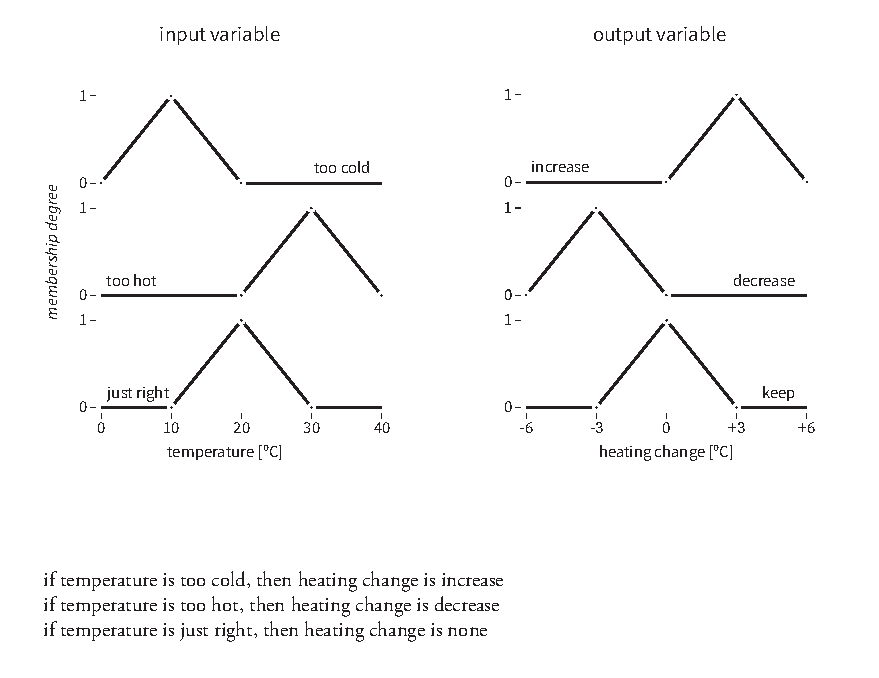
\includegraphics[width=\figurewidth]{figKnowledgebase}
	\vskip.25in
	\caption{An example of a simple fuzzy knowledge base. It describes a fuzzy rule-based system of a room temperature controller. The top part is a visual representation of the fuzzy data base. It defines two fuzzy variables, one input and one output. The input variable is the current room temperature, which is mesaured by the system via a temperature sensor. The rule base (bottom part) describes how input variables are translated into actions (output variables) via fuzzy if-then rules. In our case the action of the temperature controller is a change in room heating.}
	\label{fig:knowledgebase}
\end{figure}

In the case of animats the fuzzy data base describes how they perceive and interpret their neighbourhood and what actions they can execute to change their state and consequently the state of the universe. As such, the fuzzy data base defines the interpretation of various data obtained by the fuzzy animat's sensory system (\eg the distance to the nearest neighbour animat, heading direction of the predator animat, position of obstacles, etc.), and the actions availabe to the animat (\eg speed change, heading change, etc.). How the fuzzy animat translates the available information into actions is then defined with the fuzzy rule base.

%-----
\section{Goal: evolvable fuzzy animats}

The main goal we set ourselves for this thesis was to develop an evolutionary model, based around fuzzy logic, suitable for simulating evolution of collective behaviour inside an artificial world. As the most common hypothesis about the origins of collective behaviour states that collective behaviour might have evolved as a protection from predators \cite{cresswell2011predicting,hart2005predator,krause2002living,larsson2012why,lebarbajec2009organized,nishimura2002predator,pavlov2000patterns} it is to be expected that the direct competition between predators and prey should most likely be part of an evolutionary model that wishes to study the origins of collective behaviour. In order to properly design the model, and later evaluate it, we, for this reason, first studied the predator-prey relation and interactions in a hand-crafted model. By analysing the target selection (predation) tactics in a hand-crafted model we gained important insight into the complex world of predation tactics and prey responses to attacks. During this process we also discovered that existing models most often use basic predation tactics, whereas predators in nature adopt quite advanced approaches when hunting prey. Thus we next developed an evolutionary model where predators can tune their hand-crafted predation tactics to increase their hunting success, which could potentially give us the answer to what predation tactic is optimal for certain forms of collective behaviour or prey responses.

By using the results obtained by these two studies \cite{demsar2014simulated,demsar2015simulating} we then designed a \emph{genetic fuzzy system} for the simulation of evolution of collective behaviour. Genetic fuzzy systems \cite{cordon2001genetic,cordon2004ten,fernandez2015revisiting,herrera1996genetic,herrera2008genetic,pedrycz1996fuzzy,sanchez1997genetic} use genetic algorithms for optimizing existing or constructing new knowledge bases of fuzzy rule-based systems. Most genetic fuzzy systems focus on the optimization of hand-crafted fuzzy systems \cite{cordon2004ten,fernandez2015revisiting,herrera2008genetic}. A more demanding approach is \emph{genetic learning of fuzzy systems}, where components of a fuzzy system (the rule base, the data base, or the entire knowledge base) are not only tuned but constructed via genetic algorithms.

There are two prominent approaches for genetic rule learning -- the Michigan \cite{holland1977cognitive}, and the Pittsburgh \cite{smith1980learning} approach. With the Michigan the chromosome, as defined by the genetic algorithm, represents an individual rule and a rule base is presented by the entire population of chromosomes in a generation. The quality of the rule base (its capability of solving the problem at hand) therefore progresses through clearly defined generations. As this would lead to all animats having the same rule base we opted to use the Pittsburgh approach. With it the chromosome represents an entire rule base. This allowed us to interpret each animat individually (defined by a single chromosome) and move away from the traditional use of genetic algorithms with clear generational boundaries and closer to artificial life where there is no clear generational boundary (selection, crossover and mutation are simply part of evolution). As each animat is defined through its own chromosome, this also means that the population of animats is heterogeneous (if not by physiology by behaviour at least). This also means that the differences in individual chromosomes (rule bases) represent a source of indirect competition in the model (via their rule bases the animats compete for survival in the artificial world). One could say that prey animats in our model have to survive in an environment that is competitive in two ways. First, prey animats compete with predators for survival, and second they compete with each other to have a higher chance for reproduciton. With this and the consideration of various predation tactics we managed to design an evolutionary system that is capable of generating a wider repertoire of collective behaviours than previous approaches \cite{biswas2014causes,hein2015evolution,olson2013predator,olson2015exploring,olson2016evolution,reynolds1993evolved,sayers2009evolved,spector2003emergence,wood2007evolving}.

%-----
\section{Research methodology}

\begin{figure}
	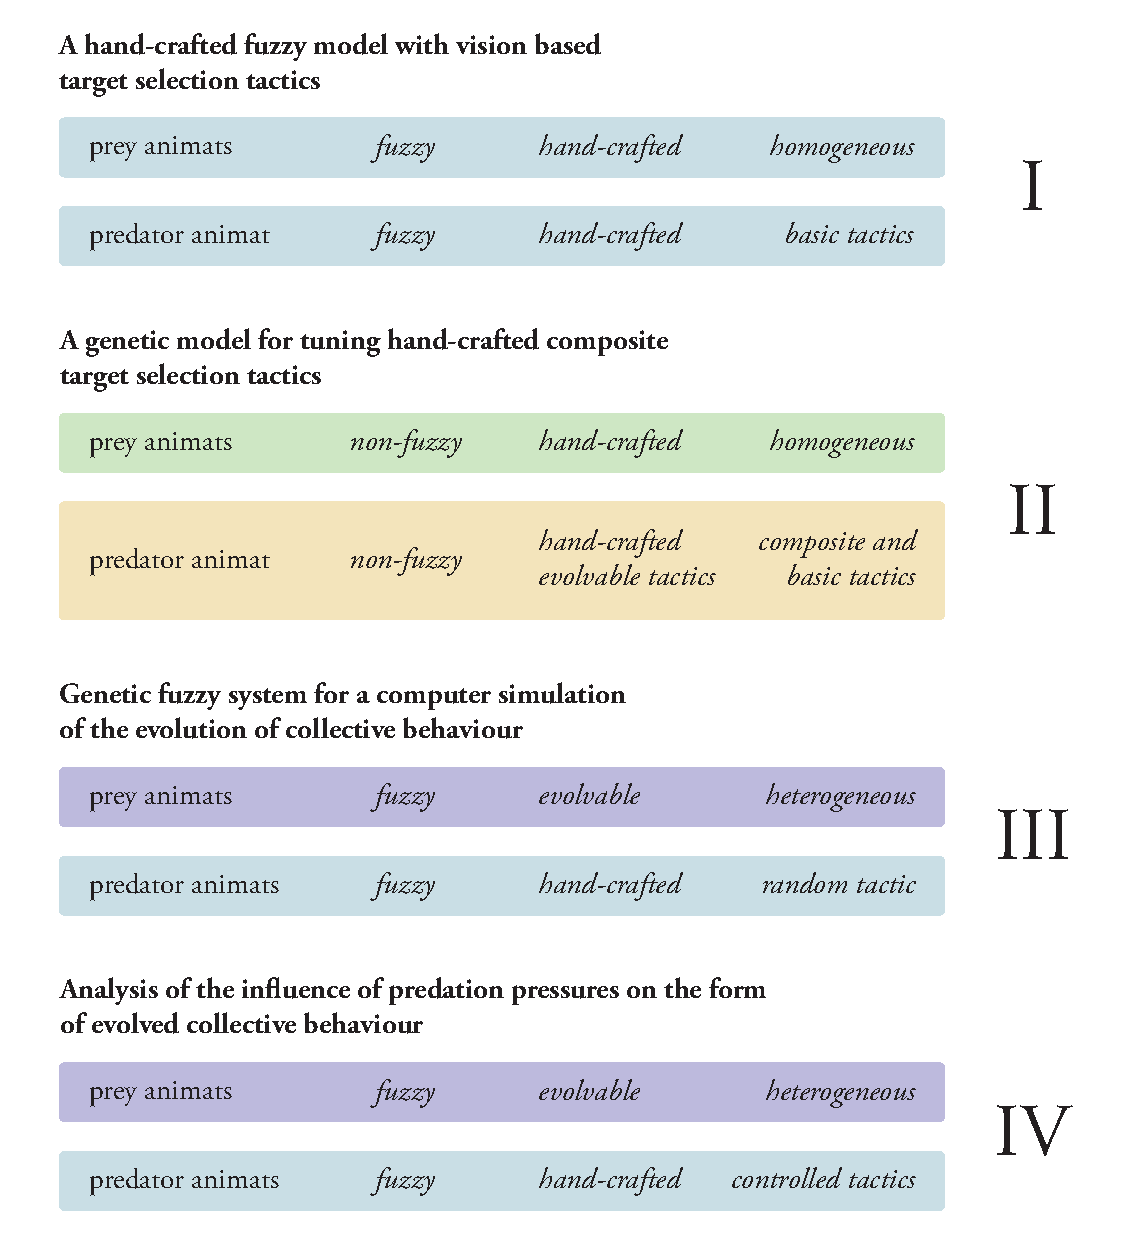
\includegraphics[width=\figurewidth]{stages2}
	\caption{A visual representation of models used in all four stages of this thesis.}
	\label{fig:stages}
\end{figure}

We split our research into four stages, each with a specific sub-goal. During these stages we developed three different individual-based models. \figurename~\ref{fig:stages} visualizes the four sub-goals and the main differences between the models used for achieving these sub-goals.

In the first model we upgraded an existing fuzzy model for computer simulation of bird flocking \cite{lebarbajec2005fuzzy,lebarbajec2005simulating}. Our principal contributions were a) the design of a perception function which mimics vision and takes into account limitations in cognitive capabilities, and b) introduction of a predator animat. The behaviour of both types of animats (the predator and prey animats) was hand-crafted. The introduction of the predator animat necessitated also the revision of the prey animats with additional drives. The behaviour of prey animats was thus based on five drives: cohesion, separation, alignment, regulate speed, and hide (escape). Cohesion, separation and alignment are visualized in \figurename~\ref{fig:drives}. The regulate speed drive implements the tendency to move with an optimal speed if there is no predator nearby. The hide drive, on the other hand, implements the tendency to escape from predators. As the behaviour of all prey animats was governed by exactly the same drives and there was no variability in their parameters prey groups were homogeneous. The behaviour of the predator was governed only by the seek (hunt) drive. A drive which implemented the tendency of predators to chase their targeted prey individual. For further details of the model refer to Chapter \ref{chap:alife}. The model was used to investigate the general hypothesis that grouping may serve as a protection from predation.

In the second stage we developed an individual-based model where the drives are implemented via differential equations (non-fuzzy). This was done to achieve comparability with previous similar models and to keep computational complexity as low as possible. The drives for both types of animats (predator and prey) were hand-crafted. In the case of prey animats the behaviour was based on previous zone-based models \cite{aoki1982simulation,couzin2002collective} and governed by the cohesion, separation, alignment and escape drive. Prey groups were homogeneous -- there was no variability in neither drives nor parameters of prey animats. The behaviour of the predator was governed only by the hunt drive. The model was used to study the evolution of composite predation tactics. To do so the parameters of each tactic were tuned with genetic algorithms, meaning that a predator was able to adapt its target selection tactic in order to increase its hunting success. See Chapter \ref{chap:ecomod} for further details of the model. 

The research in the third and fourth stage was conducted with the same individual-bsaed model, an artificial life-like genetic fuzzy system suitable for simulating the evolution of prey behaviour. The only difference was that in the third stage predators used random predation tactics while in the fourth stage the predation tactics were carefully picked to put certain evolutionary pressures on prey. Both types of animats (predators and prey) were modelled with fuzzy logic. The behaviour of predators was hand-crafted and very similar as in the first stage of our research. Predators only had one drive, the hunt drive, which implements their tendency to chase the targeted prey individual. In contrast to stage two, the predators did not adapt their behaviour through evolution. The behaviour of prey animats, on the other hand, evolved through time. Evolution of prey animats in the third and fourth stage was performed via genetic rule learning (construction of fuzzy rule bases with genetic algorithms). As we used the Pittsburgh approach for genetic rule learning each prey animat was governed by its own set of rules and could behave differently from all the other prey animats. This in turn means that prey groups were heterogeneous See Chapters \ref{chap:plos} and \ref{chap:scirep} for further details of the model. In the third stage we investigated if the model is capable of evolving a wider repertoire of collective behaviours than previous approaches, and in the fourth stage we investigated what predation pressures lead to the emergence of specific forms of collective behaviour.

%-----
\section{Scientific contributions}

We started this research with two goals in mind. The first goal was an analysis of how predator strategy and prey grouping (\eg bird flocking, fish schooling, etc.) influence prey survivability. Research devoted to achieving this gaol resulted in two scientific contributions, listed at the end of this section as a) \emph{A hand-crafted fuzzy model with vision based target selection tactics} and b) \emph{A genetic model for tuning hand-crafted composite target selection tactics} at the end of this section. Each contribution was presented on its own in the form of an original scientific paper in a renowned scientific journal. The manuscripts are included in this thesis in their entirety as Chapters \ref{chap:alife} and \ref{chap:ecomod}.

The second goal was the development of a co-evolutionary genetic fuzzy system suitable for simulating the evolution of collective behaviour. While we were working on our first goal Olson\etal \cite{olson2013critical,olson2013predator,olson2016evolution} developed a model similar to the one we set to develop as part of our second goal. They designed a probabilistic version of the animat based on Markov Networks and simulated co-evolution of predators and prey that lived in a shared environment. Results from these studies suggest that prey individuals in their case always evolved a swarming behaviour. In nature, however, collective behaviour can be observed in many forms –- swarming, milling, dynamic polarized motion, etc. Other existing evolutionary models \cite{biswas2014causes,hein2015evolution,olson2013predator,olson2015exploring,olson2016evolution,reynolds1993evolved,sayers2009evolved,spector2003emergence,wood2007evolving} were aslo unable to reproduce such a wide repertoire of collective behaviours. We view this gap between the forms of collective behaviour that can be observed in nature and those evolved via artificial evolution as the major weakness of current evolutionary models. For this reason, we decided that in lieu of focusing on co-evolution of predators and prey we will focus on designing a genetic fuzzy system capable of evolving a wider repertoire of collective behaviours. The co-evolution of predators and prey usually leads to a continuous co-adaptation of predator and prey behaviours. Needless to say such an analysis although interesting would be extremely time consuming. Thus, for reasons of simplicity the predator animat in our model is hand-crafted, \ie excluded from evolution, only prey animats co-evolve through time. Their co-evolution is the result of their direct competition with predators for survival, them being heterogeneous in behaviour, and their indirect competition where they compete with each other to have a higher chance of reproduction. This also allowed us to analyse the evolved behaviours in a more controlled manner. Research devoted to achieving our new gaol resulted in two scientific contributions, listed at the end of this section as a) \emph{Genetic fuzzy system for a computer simulation of the evolution of collective behaviour} and b) \emph{Analysis of the influence of predation pressures on the form of evolved collective behaviour} at the end of this section. Each contribution was presented on its own in the form of an original scientific paper in renowned scientific journal and the manuscripts are included in this thesis in their entirety as Chapters \ref{chap:plos} and \ref{chap:scirep}.

\subsection*{A hand-crafted fuzzy model with vision based target selection tactics} We started our research by expanding an existing fuzzy logic based model \cite{lebarbajec2005fuzzy,lebarbajec2005simulating} with predators and visual perception. Here we implemented three target selection tactics, all from the visual perspective of the predator (attack the nearest visible individual, attack the most visually isolated individual, and attack the centre of the visible group). This allowed us to study the influence of predation tactics and the impact of collective behaviour on survivability of prey individuals \cite{demsar2014simulated} . Our results suggest that for prey individuals social behaviour (governed by the separation, alignment, and cohesion drives) as opposed to individualistic (governed exclusively by the separation drive) is the most beneficial (predators take longer to capture their target). Predators, on the other hand, capture social prey individuals quicker when they attack the most visually isolated individual, but capture individualistic prey faster if they focus on the nearest prey individual.

\subsection*{A genetic model for tuning hand-crafted composite target selection tactics} In the next stage we developed an evolutionary model with which we studied composite target selection tactics \cite{demsar2015simulating}. For reasons of computational simplicity we here expanded on a known mathematical model of prey collective behaviour. This allowed us to concentrate on predator target selection tactics. We investigated the evolution of the optimal tactic with respect to prey behaving collectively and prey that performed a delayed response as a form of a defensive manoeuvre \cite{partridge1982structure}. Our results suggest that a composite tactic termed dispersing tactic, where the predator first dives deep into the group of prey and then targets the most peripheral individual, is the best tactic. This tactic seems to be the only tactic capable of at least partially diminishing the effectiveness of the preys' delayed response. This was a clear indication of potential interplay between target selection tactics and prey behaviour.

\subsection*{Genetic fuzzy system for a computer simulation of the evolution of collective behaviour} Armed with this knowledge, we developed an artificial life-like open-ended evolutionary model, where the behaviour of prey and predator individuals is governed by fuzzy logic \cite{demsar2017evolution}. In this model we focused on the evolution of prey behaviour when prey individuals face different predation tactics. We demonstrated that in this model prey individuals are capable of evolving a varied spectre of collective behaviours (swarming, milling, polarized motion, dynamic motion). Interestingly, the analysis of the evolved rule bases showed a statistically significant difference between different types of behaviour in the proportion of rules that take into account predator related information. This suggested that the predation pressures the prey are subject to during evolution might have a crucial influence on the behaviour that evolves.

\subsection*{Analysis of the influence of predation pressures on the form of evolved collective behaviour} The last step of our research was thus a controlled experiment where prey evolved under various predation tactics \cite{demsar2016balanced}. Here we let prey individuals evolve under four predation tactics, two of which according to previous research pressure prey to evolve dispersing and two pressure prey to evolve grouping. Our results suggest that antagonism in pressures, where prey are exposed to pressures for which the best response is both grouping and dispersing simultaneously, might be necessary for prey to evolve polarized movement.
